\documentclass[12pt,a4paper]{article}
\usepackage[a4paper]{geometry}
\usepackage{array}
\usepackage{hhline}
\usepackage{graphics}
\usepackage{csvsimple}
\usepackage[russian,english]{babel}
\usepackage[utf8]{inputenc}
\usepackage[T2A]{fontenc} 
\usepackage{ulem}
\usepackage{cmap}
\usepackage{makecell}
\usepackage{ifpdf}
\setlength\extrarowheight{2pt}
\setlength{\parindent}{0cm}
\newcommand{\phylentry}[6] {\\\hline\makecell{
#1\medskip\\
\hhline{|-|}
\\#2\\#3\medskip\\
\hhline{|-|}\\
{#6}}
&\makecell{#4}&\makecell{#5}}
%Syntax: \phylentry{Who}{When}{Where}{Phylosophy}{NotPhylosophy}{ETC} // currently ETC is not used
\hoffset -1.6cm 
\textwidth  16.5cm 
\textheight 24cm 
%\topmargin -1cm 
\parskip 8pt 
\setlength{\unitlength}{1cm}
\sloppy
\addto\captionsenglish{
\renewcommand{\contentsname}{{\bf CO}ntents}
\renewcommand{\refname}{Bibliography}
\renewcommand{\figurename}{Figure}
\renewcommand{\tablename}{Table}
\renewcommand{\abstractname}{Abstract}
\renewcommand{\partname}{Section}
\renewcommand{\bottomfraction}{0.5}
\renewcommand{\floatpagefraction}{0.4}
\renewcommand{\textfloatsep}{0.5cm}
\renewcommand{\intextsep}{0.6cm}
\renewcommand{\floatsep}{0.3cm}
}

\renewcommand\theadalign{cb}
\renewcommand\theadfont{\bfseries}
\renewcommand\theadgape{\Gape[4pt]}
\renewcommand\cellgape{\Gape[4pt]}
%<pics>
\newcommand{\materialist}[0]{\includegraphics{dummy-achievement.png}}%</pics>
\begin{document}
%..................................................................
\begin{titlepage}
\par 
\vspace*{-2cm}
\begin{center}
{\sf \Large
\vspace*{1.5cm}
{\Huge Семенов, 9-й семестр, 2017}\\
{ Философия, эпизод 2:}\\
{ Больше конспектов \sout{Богу} Абсолютному духу конспектов}}\\

\vspace*{2cm}
\scalebox{1.2}{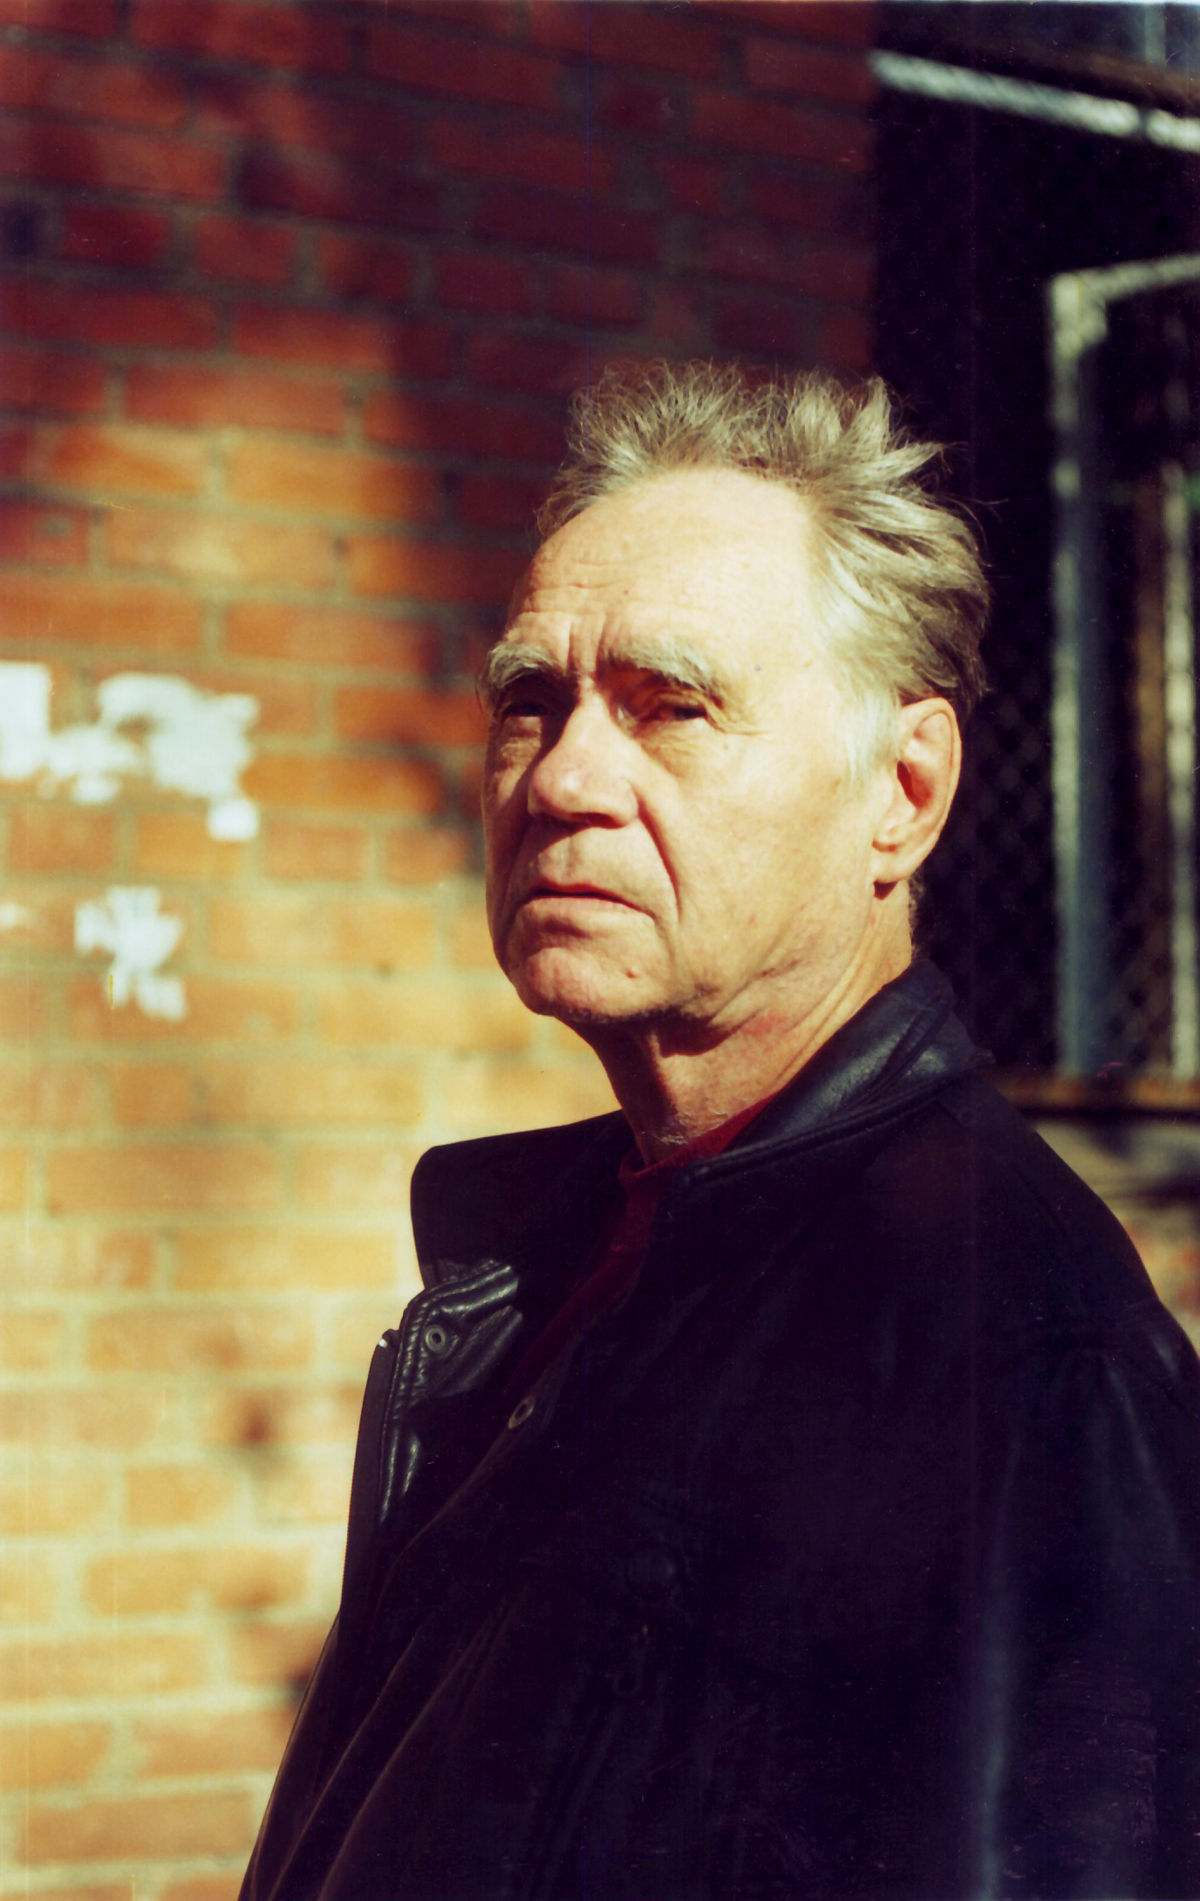
\includegraphics{thegod.jpg}} \\
{\small }
\begin{flushright}
\sl\small
by Nyaxx11k aka KingKO
\end{flushright}
\end{center}
\end{titlepage}
%..................................................................
\topmargin -1cm 
\hoffset -0.7in 
\textwidth 6.0in 
\textheight 9.0in 
\normalsize 
\pagenumbering{arabic}
%----------------
\tableofcontents
\pagebreak
%----------------

\section{Философия как наука об истине, теория познания и самый общий метод исследования}
\textit{Этот вопрос будет длинный... Итак, есть несколько взглядов на философию. Семенов придерживается того, что философия - это все же наука. Да, покукарекать за жизнь на кухне - НЕ философия.} \textbf{Философия} - это наука об истине. Конечно, это не значит, что остальные науки о заблуждении. Все науки ищут истину. Философия наука об истине именно в том смысле, что ищет истину о самой истине. Т.е. как мыслить правильно, чтобы достичь истины и не скатиться в \sout{РЕН-ТВ} заблуждение. То есть, философия есть теория познания (ака \textbf{гносеология}/\textbf{эпистемология}. Вроде, под ними многие понимают немного разные вещи, но для нас это синонимы). Ясно, что для этого философия должна разработать общий метод мышления, т.е. философия еще и наука и о наиболее общем методе познания. При этом она сама и есть этот общий метод мышления, а также и наиболее общий метод мышления. \textit{Ах да, \textbf{истина} - это то, что согласуется с действительностью, соответствие между миром и сознанием. В билетах этого не видно, но помнить будет не лишним}. 

\section{Основной вопрос философии}
"Что первично - \textbf{мир} или \textbf{сознание}?". Ну а теперь разберемся, почему же он основной. Нам необходимо дать определение мира и сознание. Обычно мы даем их через род и видовое отличие: например, студент - учащийся высшего учебного заведения. "Учащийся" - род, "высшего учебного заведения" - видовое отличие. И эта схема прекрасно работает, пока мы не дойдем до предельно общих понятий: мира и сознания, которые разделяют второе место по обощенности. На первом, конечно же, \textbf{бытие}, т.е. все. Вообще все. Соответственно, сказать, что и мир, и сознание - бытие - это ничего не сказать. Значит, определить их можно, только раскрыв их отношение: что из них первично, а что вторично. \textit{Собственно, с помощью этого вопроса классифицируют сорта философов. Главных направлений 2: \textbf{материализм} и \textbf{идеализм}. Есть еще побочные направления, у которых первично что-то третье/первичны две и более вещей/вообще неизвестно, что первично, и никогда не будет известно. Все они, правда в той или иной мере тяготеют к идеализму. Семенов даже говорил, что есть материалисты и все остальные.}

\section{Философия как мировоззрение (онтология). Натурфилософия. Философия истории.}
Итак, мы выяснили, что философия - наука об истине, а ее основной вопрос - "Что первично - мир или сознание?". Но это означает, что философия дает предельно общее мировоззрение и предельно общий взгляд на бытие. Т.е. философия - \textbf{онтология}. Раньше философия еще давала предельно общую картину мира - другие науки еще были в зачаточном состоянии, и только философия была готова дать хоть что-то. Такое учение называется \textbf{натурфилософией}. В настоящее время натурфилософия отмерла за ненадобностью. \textit{Но не онтология - она по прежнему занимается проблемами мира - теми, которые нужны для теории познания}. Но кроме природы есть еще общество - им занимаются \textbf{социальная философия} и \textbf{философия истории}. И с ними все не так однозначно, как с натурфилософией. Во-первых, есть \textbf{общественное сознание} - в широком смысле это все знание человечества; более того, сознание отдельного человека формируется в обществе \textit{(а дети-Маугли ни говорить, ни социализироваться не могут)}. Во-вторых, разные школы придерживаются разных взглядов на общество: первые говорят, что общество - только название, а на самом деле есть только взаимодействующие люди. Вторые таки признают общество. Это два направления - \textbf{социальный номинализм} и \textbf{социальный реализм} соответственно.

\section{Научная революция XVII века}
\textit{Ну, с общими вопросами разобрались, теперь поехали по философам.} Итак, наука окончательно сформирофалась в 17 в. \textit{Вообще, знание было всегда, но раньше оно было бессистемным и бездоказательным. В Древнем Египте, например, умели решать квадратные уравнения, но рецепт был получен методом тыка. Первое доказательство появилось только в 6 в. д.н.э. (привет, Фалес Милетский). Тогда, правда, наука смешивалась с натурфилософией аки нейтрино. С вытекающими отсюда переходами одного в другое. Окончательно же труЪ-наука сформировалась в 17 в.}
Ну и пробежимся по ученым того времени (спискота):

\underline{Леонардо да Винчи (1452-1519)}. Художник, изобретатель. Человек у него лишь первый из зверей, а душа не бессмертна. Один из первых \textbf{эмпириков} - ценил опыт, но и чистый эмпиризм без анализа отвергал. Развивал математику.

\underline{Николай Коперник (1473-1543)}. В книге "Об обращении небесных сфер" ввел математически обоснованную гелиоцентрическую систему. Утверждал, что это лишь способ уточнить расчеты (правда, его модель была далеко не идеальна). Говорил, что это гипотетически, боялся публиковаться. Еще бы - Церкви это ой как не понравилось. Правда, Церковь тогда была занята реформацией, а потом работа разошлась, а Коперник в тот же год благоразумно умер, и все: поздняк метяться, Земля - не центр мироздания, Бог не может жить на небесной тверди по прицине отсутствия оной. Пришлось закинуть Бога за орбиту Сатурна (то, что есть еще Уран и Нептун, никто не догадывался).

\underline{Джордано Бруно (1548-1600)}. Философ, естествоиспытатель. В работах жег не по-детски. Мир бесконечен, звезды - те же солнца, с планетами и разумной жизнью. Инопланетян что, тоже Христос создал? Вот и получается, что Бога нет. Да, в Средневековье была популярна концепция двух истин - разума и откровения. Так вот, нет двух истин - есть только истина разума, а религия - бред собачий.  Правда, мировая душа у него все-таки была, но это нечто глобальное и пассивное. У церкви с такого пригорело, однако в 1600 году на Площади Цветов во Флоренции она взяла реванш. Особый цинизм ситуации заключался в том, что костер считался гуманной казнью, так как не приводил к пролитию крови. \textit{Однако, эпопея с горящими задницами продолжается. Так, недавно поставили Джордано на этой самой Площади Цветов памятник - дескать, мученник науки, сгорел на работе, можно сказать (\textit{Вечный огонь поставьте}). Так вот, верующие раскукарекались. А узнай Джордано, что в 21 веке в одной стране поп кандидатскую по теологии защитил - сгорел бы и без дров.}

\underline{Галилео Галилей(1564-1642)}. Астроном, создатель первого телескопа (правда, подзорная труба була уже до него). Изучил Луну. Открыл спутники Юпитера (4 самых крупных). Еще и механик - опроверг положение Аристотеля о разной скорости падения тел. Изучал динамику пушечного ядра - даже в баллистики приглашали. Ну и маятник. Написал "Диалог о двух системах мира" (Птолемей vs Коперник - защищает Коперника). Написал на итальянском, а не на латыни. Слетелись инквизиторы и заставили публично отречься. Галилей отрекся (есть легенда, что в конце он произнес "И все-таки она вертится". Пруфов нет).  

\underline{Иоганн Кеплер (1571-1646)}. Опять астроном, открыл три закона обращения планет (\textit{вспомним общефиз, 1-й семестр?})

\underline{Уильям Гильберт (1540-1603)}. \textit{Не путать с Давидом Гильбертом - тот из 20-го века.} Наука и до Англии добралась. Изучал магнит, открыл джва его полюса, понял, что у Земли тоже есть магнитное поле. Еще изучал электростатику, открыл, что не только янтарь электризуется.

\underline{Уильям Горвей (1578-1657)}. Открыл кровооброщение. Основоположник физиологии и эмбриологии.

\underline{Эванжелиста Торричелли (1608-1646)}. Открыл атмосферное давление и изобрел ртутный барометр. Создал гидродинамику.

\underline{Отто фон Герике (1602-1686)}. Открыл атмосферное давление и изобрел ртутный барометр. Создал гидродинамику.

\underline{Роберт Бойль (1627-1691)}. Открыл закон имени себя-Мариотта. Создал научную химию.

\underline{Эдм Мариотт (1620-1684)}. Открыл закон имени Бойля-себя. Создал французскую академию наук.

\underline{Христиан Гюйгенс (1629-1691)}. Открыл кольца Сатурна, создал маятниковые и пружинно-балансирные часы. Моряки сказали спасибо, ибо без них долготу корабля фиг определишь. Создал теорию маятника и волновую теорию света.

\underline{Антон ван Левенгук (1632-1723)}. Изобрел микроскоп. Открыл бактерии, изапилил микробиологию. \textit{А однажды плюнул под микроскоп. Посмотрев на зоопарк полости рта, стал чистить зубы еще до того, как это стало мейнстримом.}

\underline{Роберт Гук (1635-1705)}. Закон имени себя.

\underline{Исаак Ньютон (1642-1716)}. 3 закона имени себя + закон всемирного тяготения + матан, независимо от Лейбница. Сделал механику точной наукой. Топил за корпускулярную теорию света - \textit{создатель квантмеха (нет)}
 
На этом спискота все. Итого 12 ученых. А если в общем - ученые стали ставить эксперименты (систематические), юзать приборы - всякие теле-микро-скопы, баро-термометры, часы. Появились обсерватории. В Англии Карл II запилил первую академию наук - т.н. "Королевское общество" (1662). Потом тренд подхватили Франция, Пруссия, а там и в Россию завезли. Ученые стали делать доклады, а сборники этих докладов стали первой научной прессой. Потом, когда ученых стало побольше, уже и нормальная периодика пошла. Появилось и научное мышление. Чудеса наука не рассматривала. Да, гнать на церковь по-прежнему было накладно, но это уже шаг вперед . Появилась концепция \textbf{детерминизма} - учения о всеобщей причинности и предопределенности событий. Потом и теорвер появился. Он с детерминизмом прекрасно уживался - все случайности проистекают из нашего недостаточного знания, а на самом деле все предопрелелено. Тут нужно упомянуть Лапласа с его демоном. Если демон знает коориднаты и скорости всех тел, а также имеет бесконечную разрядность и производительность, он сможет просчитать все события в нашем мире. Такой вот \textbf{механистический детерминизм}. \textit{Правда, квантовая механика похоронила абсолютный детерминизм, но в пропатченных вариантах он жив}.
%Smth else?

\section{Западноевропейская классическая философия XVII - первой половины XIX вв. Эмпиризм и рационализм.}
Итак, окончательно сформировалась наука. И тем самым у философов появилась пища для ума. Откуда берется научное знание? Как мыслить так, чтобы полученные теории действительно работали? \textit{Тут нужно сказать, что есть два вида знания - \textbf{житейское} и \textbf{научное}. Первое - бессистемное и бездоказательное, полученное в ходе повседневной человеческой деятельности. Второе же и системное, и обосновывается. Например, счет на пальцах у древних людей - это житейское знание. А аксиоматика Пеано - научное}. Надо сказать, еще Бэкон (который Роджер) выделял три источника знания - авторитет, ум и опыт. То, что авторитет может ошибаться - и так понятно. А с умом и опытом сложнее. И тут возникли два направления - \textbf{эмпиризм} и \textbf{рационализм}.

Эмпиристы утверждают, что единственный источник знания - опыт (Р. Бэкон, к слову, тоже придерживался этой мысли). \textbf{Априорного}, т.е.полученного без опыта знания у них нет - только  \textbf{апостериорное}. Да, самое главное: а что есть \textbf{опыт}? Ну, опыт бывает житейский и научный. С ними все примерно так же, как и со знанием. Житейский получается в ходе человеческой практики - хочешь, чтобы что-то заработало - делай так-то, а так-то, наоборот, не делай. Научный - продуманный, системный, знание, полученное в ходе него, фиксируется в суждениях, т.е. становится \textbf{фактом}. Нельзя сказать, что все эмпирики отвергают разум: многим он нужен для обработки экспериментальных данных в теории. Т.е. сначала эмпирический уровень знания, а потом и теоретический. Есть же и \textbf{сенсуалисты} - у них в разуме нет ничего, чего не было бы в чувствах (\textit{ага, многие из вас видели отдельные атомы?}).

Рационалисты, напротив, говорили, что априорное знание есть, и более того, оно даже круче апостериорного: опыт может раз сработать, два сработать, а на третий раз слажать, а вот что доказано умом - то работает всегда.

А где же истина? А она, как всегда, где-то рядом. Действительно, мир дан нам только в наших чувствах - правы сенсуалисты. Но разум в состоянии раскрывать закономерности, находить причинно-следственные связи и создавать реально работающие (разумеется, с определенной точностью и в определенных границах) теории - правы рационалисты. Так что, все эти направления - это, как правило, раздувание одной стороны истины в ущерб другим.

\section{Философия Френсиса Бэкона}
\underline{Френсис Бэкон (1561 - 1626)}. Англичанин. Не был старшим сыном, а потому остался без земли в наследство. Пришлось кончить Оксфорд и работать адвокатом. Был близок ко Двору. В 1603 оборвалась жизнь Елизаветы I, а вместе с ней и династия. Взошел на престол Якоб I (по Шотландии уже Якоб VI; если быть точнее, James VI). При нем Бэкон стал лордом-хранителем печати, а потом (16!8) и лордом-канцлером. Правда, потом карьера его пошла под откос: в 1621-и парламент, решив насолить королю, привлек Бэкона за взяточничество и злоупотребление властью. Коррумпированный лорд получил 40к штрафа, запрет на работу в сфере политики и камеру в Тауэре "до освобождения". Король, правда, отменил первые два наказания, потом и ко двору допустили, но осадочек остался. В итоге, отсидел Бэкон только два дня (\textit{привет, Васильева}). Карл I, сев на трон, и вовсе хотел восстановить Бэкона в должности, но тот отакзался.

Бэкон писал книги. Нам нужен его опус 1620-го года \textbf{"Новый органон"} (\textit{В пику "старому" Органону - набору работ Аристотеля по логике.}). Наука у него - высшая форма знания о природе.
Не нравилось Бэкону, что как-то на практике теория не шибко юзается.  Он выдвинул три тезиса:
\begin{enumerate}
\item Объект научного познания - природа.
\item Задача науки - познавать природу.
\item Цель - подчинить природу человеку.
\end{enumerate}
Ну и конечно, для познания нужен метод. Его Бэкон и хотел запилить. Итак, начнем с его четырех препятствий для ученого ака \textbf{четырех идолов}:
\begin{enumerate}
\item Идол рода: в мышление вносят искажения природа человека и тело человека . 
\item Идол пещеры: знание ограничено. Всегда кажется, что все уже открыли.
\item Идол площади/(\textit{у анкапов сейчас подгорит})рынка - существует множество точек зрения, в том числе популярных и неверных. Надо бы  от них отказатья, а общественное мнение не дает.
\item Идол театра: древние мыслители и авторитеты. Они могут ошибаться.
\end{enumerate}

Источник знания - чувства. Таки да, \textbf{сенсуалист}, но не радикальный: знание - не просто набор фактов. Ученых делил на три категории:
\begin{enumerate}
\item Муравьи. Просто таскают факты в муравейник.
\item Пауки. Тянут из себя теории без опоры на факты.
\item Пчелы. А вот эти годные: сначала собирают факты-нектар, а потом фигачат из них мед-теорию. \textit{И летают.}
\end{enumerate}

Аристотель в Органоне изучал только дедукцию. В Новом же Органоне разбирается индукция и построенная на ней логика. Для этого есть методы \textbf{сходства}/\textbf{различия}/\textbf{выявления причин}. Ну и до кучи еще термины: \textbf{анализ} - расчленение на части; \textbf{синтез} - соединение в целое. Семенов приводил пример: анализ - тяжелое, пластичное, желтое, синтез - золото. \textbf{Форма} у Бэкона - законы и сущности явлений. У него 19 форм движения - механистическим редукционизмом не страдал.

\section{Философия Рене Декарта}
\underline{Рене Декарт(1596 - 1650)}. Он же Картезиус на латыни. Человек и система координат. Учился в Иезуитском колледже, потом дропнул и пошел работать. Был из дворянского рода, но младшим сыном. Как наемник пошел в армию, причем сразу в офицеры (дворянин же). Опять дропнул и уехал в Голландию философствовать. В Голландии тогда прошла буржуазная революция, вероисповедание свободное, Республика семи провинций. Запилил книжку "Размышление о методе \textit{<там полное длинное заглавие, но и так сойдет>}". В этой книжке - 4 правила для исследователя:
\begin{enumerate}
\item За основу берутся очевидно истинные положения.
\item Дальше они \textbf{анализируются} - расчленяются на составные части.
\item А потом \textbf{синтезируются} воедино, от простого к сложному.
\item Всегда проверяется, не упущено ли что-либо важное.
\item ?????????
\item PROFIT
\end{enumerate}
Источники знания у него:
\begin{enumerate}
\item Самое главное - априорные идеи (\textit{ну вы чувствуете, какой \textbf{рационалист}?}). Они и так очевидны.
\item Интуиция.
\item Дедукция.
\end{enumerate}
Да, априорные идеи. Во-первых, я мыслю, а следовательно существую. Т.е существует мыслящая субстанция.
Во-вторых, существует Б-г - это врожденная идея. В-третьих, есть вещи - о них говорит Б-г (\textit{блин, ну Декарт}). А значит есть протяженная субстанция. Мир у него существует в пространстве и времени, но они - такая же материя. Это \textbf{реляционная} концепция, в пику \textbf{субстанциональной}. Да, Декарт \textbf{дуалист} - у него и мир первичен, и сознание. Да не совсем - их сначала создал Б-г, который все-таки скорее сознание. Правда, потом Б-г на мир забил (\textbf{деизм-с}), и они как бы оба первичны, но слив идеализму засчитан. Планеты и звезды у него появиись из облака мельчайших частиц (за подробностями уже к Канту с Лапласом). \textbf{Механист}, и как сказано ранее, \textbf{деист}: Бог создал законы, а дальше все само собралось. Животные у него - просто куски материального мира, управляемые рефлексами (уже разделял врожденные и приобретенные). А вот человек - единство души и тела.

\section{Философия Томаса Гоббса}
\underline{Томас Гоббс (1588 - 1679)}. Родился в семье служащего. Тоже кончил Оксфорд, дальше пошел в домашние учителя для богатых людей (Это весьма частая завязка биографий). Путешествовал по Европе.  Изучил "Начала" Евклида. Проникшись строгостью математики, захотел того же от других наук. Написал труд "О гражданине" - книгу об обществе. Во Франции сблизился с английской королевской семьей. \textit{Стопчто?! С английской королевской семьей во Франции?! Ну, там было так... Захотел Карл I запилить новый налог в 1641-м. образ парламент. А блэд  пэрлэмэнт потребовал наказать коррупционеров. Лорду-канцлеру пришлось отрубить голову. Не успокоились. Началась ревоцюция, гражданская война. Короля поймали, он бежал, потом снова поймали, судили, и в итоге он, как и лорд-канцлер, попрощался с головой. А вот семья таки успешно завела трактор.
% Кстати, Гоббс критиковал применение силы в работе "О гражданине", а так как Кромвель и Ко именно что применением силы и занимались,  пришлось Гоббу валить -- PROOFS NEEDED
} Так вот, Гоббс с ними сблизился, потом поссорился. Накатал "Левиафана" - там топил за сильное государство. Там же вводит концепцию общественного договора. Кромвелю, который к тому моменту сосредоточил власть в своих руках, понравилось. А потом Кромвель умер. Король вернулся, то теперь его повязали по рукам и ногам конституцией. 

Итак, это была биография Гоббса. А тепеть его взгляды. Вообще, они изложены в трех его работах: "О теле", "О человеке", "О гражданине". \textbf{Материалист}. Значение науки для него огромно. Она строится на фактах, но их необходимо переработать в теорию. А для этого, опять-таки, нужен метод. \textit{Ах да, теологию высмеивал. Так ей и надо.} В его терминологии чувствуется тяга к матану. Так, он все "складывал" и "вычитал". Ввел понятие \textbf{метки} - вещи, заставляющей вспомнить о чем-либо, и \textbf{знака} - вещи,метки, юзаемой в общении (\textit{слова, например}). Крайний \textbf{номиналист}, хотя и  сбивался к умеренному. Мир у него - гиганская совокупность тел - телесная субстанция (\textit{чувствуется материализм}) - она вечна. Декарта критиковал - мышление - свойство высокоорганизованной субстанции, а не сама субстанция. Мир существует во времени и пространстве. Есть и движение, но тут Гоббс - \textbf{механистический редукционист}. Как почти неизбежное следствие этого, \textbf{абсолютный детерминист}, отрицал теорию \textbf{двух истин}, чудеса, \sout{заговор жидомасонов с иллюминатами и плоскую Землю}. Отрицал даже свойства типа цвета, вкуса и запаха - типа это порождение сознания (\textit{Демокрит, привет}). Мир имеет двоякое бытие - сам по седе и в сознании. В сознании он отражается. 

А теперь, как двигать науку. Тут все почти то же самое: анализ, синтез и дедукция. Он заимствует идеи рационализма- геометрия, например, у него дает общее знание, ибо не опирается на опыт. Науки он делил на индуктивные (опирающиеся на эмпирические факты, например, физика) и дедуктивные (например, геометрия или наука об обществе).

Люди у него сначала жили без норм и понятия о собственности. Каждый сталкивался с каждым - "Война всех против всех". Во избежание этого, были запилены государство и собственность. Формы государства три - республика, аристократия и абсолютная монархия (Гоббс именно ее и уважает). Атеист, но религия у него нужда, дабы \sout{быдло} народ не бунтовал.

\section{Философия Баруха Спинозы}
\underline{Барух (Бенедикт) Спиноза (1632 - 1677)}. Родился в Республике семи провинций (нынешняя Голландия). Родился в Амстердаме, в гетто - таки евrей. Учился в еврейской школе, изучал Ветхий завет. Думали, способный малый, богослов будет - ан нет, малый действительно оказался способный - положил на синагогу свой обрезанный и ушел в Латинскую школу. Ему предлагали хотя бы делать вид, что иудаист - отказался. Устроили сначала малое, а потом и великое отлучение(1656) - выперли из общины. Пошел к ван Эйдену, но евреи добились его изгнания из города как безбожника. Голландия, конечно, была веротерпимой, но вовсе не атеистотерпимой. Так и осел Спиноза в деревне. Шлифовал линзы и философствовал. В 1673 курфюрст Фальце пригласил в Гейдельбергский университет. Зарплата - во! Единственное - просьба поосторожнее высказывать мнение. Но Спиноза сломал стереотипы о евреях и атеизм на шекели не променял. Французы предложили одну из работ посвятить королю. Отказался - "Я свои работы посвящаю только истине!"

Сначала был \textbf{дуалист}. Потом - \textbf{монист}. Субстанция у него  - это Б-г (\textbf{пантеист}). Субстанция вечна, бесконечна в пространстве и времени, неделима и не состоит из частей, а еще она мыслит. Природу делит на \textbf{производящую} (собственно, Б-г) и творимую. Проявления субстанции носят название \textbf{модусов}. Это - вещи, они не вечны, движутся (\textit{Но субстанция неподвижна, аки у Парменида с Зеноном}). \textbf{Абсолютный детерминист} - есть всеобщая предопределенность. Но и свобода есть - это осознанное и добровольное подчинение необходимости.

Выделял четыре формы познания:
\begin{enumerate}
\item Знание понаслышке
\item Бессистемный опыт
\item Рассуждение
\item Интуиция - рр-раз, и допер. Интуиция не обманывает. Но и в мистику Спиноза не скатывается. Просто способность человека, которую он не осознает. 
\end{enumerate}
Таки \textbf{рационалист}. Религия возникает от невежества и страха перед природой, и должна быть побеждена просвещением. Наука опирается на факты. История в том числе, и к источникам же нужно относиться критически - когда создан, кем, откуда это кто-то узнал о событии. В принципе, Лоренцо Валла об этом уже говорил. Спиноза так покритиковал Библию. В частности, показал, что Пятикнижие Моисеево ака Тора написана точно не Моисеем. Причина проста: там есть описание смерти Моисея. А зомби вроде как в Библии отсутствуют (Лазарь не в счет, тем более что абилка на воскрешение только у Иисуса была).

\section{Философия Готфрида Лейбница}
\underline{Готтфрид Вильгельм Лейбниц (1646 - 1716)}. Родился в Лейпциге. Отец - профессор морали. Говорят, корни у Лейбница славянские (\textit{мамкиному националисту на заметку}). Работал в области науки и философии. Запилил счетную машину. Германия тогда еще не была буржуазной страной. Буржуазия была осторожной и шла на компромиссы. И философия Лейбница тоже. Хотел он науку с религией помирить. \textbf{Мех. редукционизм} не уважал. А вообще философия у него интересная. Он, как и Декарт, маргинал - не материалист и не идеалист (\textit{ну, как сказать не идеалист...}). Он \textbf{плюралист} - первично дофига всего. Его учение - \textbf{монадология}. Монада - субстанция; каждая сама по себе. Их бесчисленное множество. Они существуют вне времени и пространства, замкнуты на себя и не связаны друг с другом. Они неуничножимы, а, нет, есть высшая монада, которая может создавать и уничтожать остальные. Кто она? Б-г. Короче, \textbf{объективный идеализм} так и зияет через дыры в теории. Монады движутся и действуют. Без связи друг с другом - Б-г их откалибровал так, что достиг гармонии. Монады делятся на три сорта:

\begin{enumerate}
\item Голые. Неразвытые, без восприятия.
\item Души - уже есть восприятие ака \textbf{перцепция} (как животные).
\item Духи - у них и сознание ака \textbf{апперцепция} есть.
\end{enumerate}
Материя же - сложная субстанция из простых субстанций, т.е. монад. Материй у него два сорта. Первый - протяженная масса.
Второй - активная материя - находится в движении. В механицизм Лейбниц, как и было сказано ранее, не впадал. У него и появление качеств, и развитие - это формы движения.  Всякий покой только относителен. Есть и принцип сохранения силы - она не появляется и не исчезает, а только переходит из одного состояния в другое. В теории познания Лейдниц ставит во главу угла мышление - \textbf{рационалист}. Истин две (\textit{не путать со схоластикой!}) - истина разума, и случайная истина как результат эксперимента. А еще Лейбниц считал, что живет в наилучшем из возможных миров. И оправдывал Б-га (\textbf{теодецея}) - "Бог создал добро, а его нет без зла".


\section{Философия Джона Локка}
\underline{Джон Локк (1632 - 1704)}. Кончил Оксфорд. Отец участвовал в революции на стороне Парламента, был там капитаном. После Оксфорда Локк пошел преподавать, потом познакомился с лордом Эшли (ака графа Шефтсбери), оппозиционером. Стал его врачом. Когда лорд стал лорд-канцлером, Локк стал его секретарем, а когда началось преследование, свалил в Голландию. Вернулся только после т.н. "Славной революции", когда очередного короля (на этот раз Якова II) низложили. Славная - значит бескровная. 

В 1690 г. пишет "Опыт о человеческом разуме". \textbf{Эмпирист} - все  знание апостериорно, а человек рождается \textbf{tabula rasa} (лат. "с чистого листа"). Опыт у его двух сортов: \textbf{внешний} (предмет подествовал на органы чувств) и \textbf{внутренний}, ака опыт \textbf{рефлексии} - наблюдение разума за самим собой. \textit{Вообще, назвать опытом рефлексии мышление - значит маскировать рационалистические мысли.} От них появляются простые чувственные и рефлексивные идеи, которые уже превращаются мозгом в более сложные. Качества у него тоже двух видов - первичные (объем, вес и т.д.) и вторичные (цвет, вкус, звук и т.д.). Про них будет далее. Субстанция у него есть \textbf{телесная} и \textbf{мыслящая}. Сущность вещей у него непознаваема. Есть три формы познания - \textbf{интуиция} (очевидное) (\textit{Локка так и тянет в рационализм}), \textbf{демонстративное} познание (доказуемое) и \textbf{опытное/сенситивное} (ограничное). А еще он \textbf{деист}.

\section{Учение Джона Локка о первичных и вторичных качествах}
Качества у Локка двух видов - \textbf{первичные} (объем, вес и т.д.) и \textbf{вторичные} (цвет, вкус, звук и т.д.). Первые объективны и неотделимы от тел, вторые субъективны и в том виде, в котором человек их воспринимает, в телах не существуют.
% 
\section{Философия Джорджа Беркли}
\underline{Джордж Беркли (1685 - 1753)}. Окончил Тринити-колледж. Священник. Стал домашним священником одного дипломата. Потом и епископом стал. 

Решил, что материализм - фундамент атеизма, а посему, чтобы разрушить атеизм, надо развенчать материализм. \textit{Семенов против смешивания религии с идеализмом, кстати. Идеализм  все же научная теория (пусть даже Семенов считает ее неверной), а религия бездоказательна и включает в себя культ. Не поклонялись же философы Абсолютному духу.} Так вот, для пропаганды ХГМ Беркли выкатил прямо-таки антипод материализма - \textbf{субъективный идеализм}. Согласно нему, сознание не просто первично, а мир существует исключительно в моем сознании \textit{(Так и говорим - "в моем сознании". Не "в сознании Беркли")}. До кучи \textbf{крайний номиналист} - нет общего, и материи нет, ибо она - общее (\textit{еще бы она была - это сугубо безбожный материалистический термин, обозначающий объективное бытие}). Все состоит из чувств - ведь мир только в сознании. Быть - значит быть воспринимаемым. Вот и до \textbf{солипсизма} докатился. Манямир в сознании Беркли трещал по швам. Сначала, ему пришлось ввести мыслящих духов - иначе бы предметы пропадали, когда Беркли отворачивался от них и/или спал. Мыслящие духи, конечно воспринимали предметы, препятствуя их исчезновению, но исключительность моего сознания${}^\mathtt{TM}$ оказалась подорвана. Дальше, каждый безбожник-материалист, да и вообще каждый философ, еще не дофилософствовавшийся до психбольницы, не пытался наесться воображаемыми, скажем, яблоками. Но в Берклимире-то восприятие/представление и есть сам предмет! Пытавшись покукарекаться с тем, что представление какое-то бледное по сравнению с восприятием, Беркли в конце концов ввел-таки Бога, который должен был отделять одно от другого. \textit{Казалось бы, наличие Б-га доказано и материализм-атеизм побежден. Вин? А вот и нет, фейл. Дело в том, что такой Б-г - самый настоящий Абсолютый д-х. Вот и развился субъективный идеализм в свою противоположность - в объективный. А что, неплохая иллюстрация диалектики.} А еще Беркли писал книги. 1710 - "Трактат о принципах человеческого знания",  1713 - "Три диалога между Гиласом и Филонусом".

\section{Философия Давида Юма. Обоснование им феноменализма (агностицизма).}
\underline{Давид Юм (1711 - 1776)}. Шотландец, сын дворянина. Написал историю Англии (8 томов!) и историю религии. На интересует его "Трактат о человеческой природе". В двух частях. В первой исследовал познание, в второй - эмоции. в 40-м году дописал третью часть - учение о морали. в 48-м было запилено второе издание первой части - "Исследование человеческого познания". 

\textbf{Эмпирик} - единственный источник знания - опыт. Тут он заодно с Локком - есть \textbf{перцепция} и \textbf{рефлексия}. О рефлексии почти ничего не писал. Чувственный опыт делится на \textbf{представления} ака \textbf{идеи} - они бледные и тусклые, и на \textbf{впечатления/восприятия}, которые делятся на \textbf{простые} - отдельные чувства, и сложные - (восприятие целиком отдельного предмета). На вход подается чувственный материал, а дальше он обрабатывается - ищется:
\begin{enumerate}
\item Сходство.
\item Смежность (близость в пространстве).
\item Причинность.
\end{enumerate}
И знание тоже двух типов - частные и недоказуемые \textbf{факты}, и всеобщее и доказуемое знание, получаемое развертыванием идей (как математика).

Юм создал \textbf{агностицизм} - учение, в котором утверждается неразрешимость основоного вопроса философии. Объяснял он это так: вещь познана - значит она вошла в наше сознание. Следовательно, то, что в сознание не вошло (например, мир - если мы его знаем, то он в сознании)  -то непознаваемо. Это не значит, что ничто не познаваемо - содержание своего сознания мы знаем. На основной вопрос Юм дает три гипотетических ответа:
\begin{enumerate}
\item Да, есть вещи вне сознания
\item Нет, есть только наши представления
\item Нет, Б-г вкладывает мир в наши ощущения
\end{enumerate}

С точки зрения формальной логики не подкопаешься. \textit{Но Юма можно опровергнуть созданием теории, то есть с помощью разумного мышления. Однако, отпочковавшиеся от агностиков \textbf{позитивисты}, которые сейчас доминируют, такие доказательства не признают (а иногда и разум).}

\section{Основные идеи века Просвещения}
\section{Возникновение первых научных периодизаций мировой истории и концепции прогресса (человеческого общества Адам Фергюсон, Адам Смит, Жак Тюрго, Жан Кондорсе).}
\section{Жан-Жак Руссо, Морелли, Габриэль де Мабли}
\section{Географический детерминизм. Ш. Монтескье.}
\section{Демографический детерминизм.  К.А. Гельвеций и А. Барнав.}
\section{Вольтер}
\section{Жан Мелье}
\section{Борьба французских материалистов XVIII в. против идеализма и религии}
\section{Учение французских материалистов XVIII в. о природе. Их механицизм и абсолютный детерминизм}
\section{Теория познании французских материалистов}
\section{Учение французских материалистов XVIII в.  об обществе и истории}


\section{Немецкая классическая философия}
\section{Иммануил Кант.  Жизнь и развитие его философской мысли.}
\section{Учение Иммануила Канта о ноуменах (вещах в себе) и феноменах (вещах для нас)}
\section{Априоризм Иммануила Канта}
\section{Иммануил Кант о синтезе чувственности и рассудка}
\section{Открытия Иммануила Канта. Рациональное зерно, содержащееся в его гносеологической концепции.}
\section{Иммануил Канта о разуме. Антиномии разума.}
\section{Жизнь и философия Иоганна Готлиба Фихте}
\section{Жизнь и философия Фридриха Вильгельма Йозефа Шеллинга}

\section{Георг Вильгельм Фридрих Гегель. Его жизнь и основные работы.}
\section{Проблема истины в "Феноменологии духа" Георга Гегеля}
\section{Открытие Георгом Гегелем мышления как объективного процесса. Гегелевская диалектика.}
\section{Философская система Георга Гегеля}
\section{Наука логики Георга Гегеля}
\section{Философия природы Георга Гегеля}
\section{Философия духа Георга Гегеля}
\section{Противоречие между методом и системой в философии Георга Гегеля}
\section{Великая Французская революция и крах волюнтаризма.  Философия истории Георга Гегеля. }

\section{Раскол в школе Г. Гегеля. Младогегельянцы (Давид Штраус, Бруно Бауэр).}
\section{Антропологический материализм Людвига Фейербаха}
\section{Кризис материализма на рубеже XVIII–XIX вв.}
\section{Исторические предпосылки возникновение марксизма. Основные части марксизма.}
\section{К. Маркс и Ф. Энгельс как создатели марксизма. Эволюция их взглядов.}
\section{Философская и обществоведческая мысль в поисках объективного источника общественных идей. Французские историки эпохи Реставрации.}
\section{Философская и обществоведческая мысль в поисках объективного источника общественных идей. Открытие экономических отношений и возникновение политический экономии.}
\section{Философская и обществоведческая мысль в поисках объективного источника общественных идей. Выделение основных эпох истории цивилизованного общества.}
\section{Философия истории А. Сен-Симона.}
\section{Экономический детерминизм Ричарда Джонса.}
\section{Создание материалистического понимания истории и его основные понятия.}
\section{Возникновение диалектического материализма и его отличие от всех предшествующих материалистических систем.}
\section{Возникновение диалектического материализма и его отличие от предшествующих материалистических систем}
\section{Классическая и неклассическая западноевропейская философии Нового времени. Их отличие и особенности их развития.}
\section{Основные течения западноевропейской постклассической философии: иррационализм, первый, второй и третий позитивизм, постпозитивизм, постмодернизм}

\end{document}
